\documentclass[8pt]{beamer}
\usepackage{lipsum}
\usepackage{epsfig}
\usepackage{amsmath}
\usepackage{amssymb}
\usepackage{multicol}
\usepackage{graphicx,url}
\usepackage[german, english]{babel}
\usepackage[utf8]{inputenc}

%\usepackage{fancybullets}
\newtheorem{Def}{Definition}
\definecolor{SectionCol}{rgb}{1.0,0.6,0.0} %orange

\subtitle{W4 CAA Scripting Languages Hackathon I}
\title{Can you code this?}
%Título do projeto

\author{Clemens Schmid$^{1}$, Martin Hinz$^{2}$, Carolin Tietze$^{3}$}
%nome dos autores

\institute
{$^{1}$ Römisch-Germanisches Zentralmuseum Leibniz-Forschungsinstitut für Archäologie: Mainz, Rheinland-Pfalz, clemens@nevrome.de; $^{2}$ Institut für Archäologisches Wissenschaften, Universität Bern, martin.hinz@iaw.unibe.ch; $^{3}$ Institut für Klassische Altertumskunde, Christian-Albrechts-Universität zu Kiel, ctietze1991@gmail.com
}
%Nome e endereço da Instituição

% Exibe os logos (direita e esquerda)
% Procure usar arquivos png ou jpg, e de preferencia mantenha na mesma pasta do .tex
%%%%%%%%%%%%%%%%%%%%%%%%%%%%%%%%%%%%%%%%%%%%%%%%%%%%%%%%%%%%%%%%%%%%%%%%%%%%%%%%
%%% Begin of Document
\setbeamertemplate{footline}[text line]{%
  \parbox{\linewidth}{\vspace*{-8pt}{\bf CAA 2019} Check Object Integrity - 47th CAA - 23-27 April 2019\hfill\insertpagenumber}}


\begin{document}
%define conference poster is presented at (appears as footer)

\begin{frame}
\titlepage
\begin{flushright}

\includegraphics[height=1cm]{images/49449374.png}
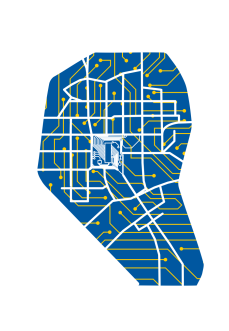
\includegraphics[height=1cm]{images/front_20180624.png}
\end{flushright}
\end{frame}



\begin{frame}
\section{General Information}

\begin{itemize}
\item A \textbf{repository} with all information and data for this workshop is available at \newline \url{https://github.com/sslarch/caa2019_hackathon}
\item 2-4 \textbf {groups} are formed on site according to framework preference and skill levels (\textit{Unconference style}).
\item We have until \textbf{4pm} to work together. Breaks can be taken as you wish, but a joint lunch break at 12:30pm might be a good idea. 
\item It is not necessary to complete all possible tasks. Work as far as you can go. Most tasks are independent of each other, so you can skip boring ones. This is \textbf{NOT} an exam.
\item All results must be submitted in one \textbf{reproducible report} with all code and plots. This can be rendered from IPython Notebook, Rmarkdown, Latex, etc. or compiled manually. Ideally the report is submitted as a Pull Request to the hackathon repository on github. The file(s) should be added to the \emph{reports} directory.
\item The organizers of this workshop are available for questions and advice. They are able to assist you with problems as far as they are familiar with your toolset.

\end{itemize}

\end{frame}

\begin{frame}

\section{Dataset}

The data for this excercise --- \verb|Michelsberg| --- are taken from the R package \verb|archdata| (Carlson/Roth 2018). It is a features by types table of abundance data on vessel types in archaeological features of the Younger Neolithic Michelsberg Culture from Belgium, France and Germany by Birgit Höhn (2002). The 109 observations/lines represent individual features (pits, ditches, etc.) from sites. For each feature we have information about 42 variables/columns. These include identifiers, classified pottery type counts, phase attribution and site coordinates.

\end{frame}
\begin{frame}
\bigskip

\textit{From} \verb|?archdata::Michelsberg:|

\begin{multicols}{3}

\begin{tiny}

\begin{itemize}
\item id: Unique identifier (categorical, integer)
\item site\_name: Name of site (categorical, character)
\item catalogue\_nr: Number in catalogue of Höhn (2002) (categorical, integer)
\item feature\_nr: Number of the archaeological feature (categorical, numeric)
\item to3: Pot/vessel type 3 count
\item f4: Bottle type 4 count
\item b2: Beaker type 2 count
\item to2: Pot/vessel type 2 count
\item b3: Beaker type 3 count
\item b7: Beaker type 7 count
\item kw5: Carinated bowl type 5 count
\item vg1: Storage vessel type 1 count
\item vg2: Storage vessel type 2 count
\item t4a: Tulip beaker type 4a count
\item kw2: Carinated bowl type 2 count
\item kw4: Carinated bowl type 4 count
\item b5: Beaker type 5 count
\item t3b: Tulip beaker type 3b count
\item f3: Bottle type 3 count
\item kw3: Carinated bowl type 3 count
\item kw1: Carinated bowl type 1 count
\item b6: Beaker type 6 count
\item to1: Pot/vessel type 1 count
\item b1: Beaker type 1 count
\item t3a: Tulip beaker type 3a count
\item vg4: Storage vessel type 4 count
\item ks2: Conical bowl type 2 count
\item ks1: Conical bowl type 1 count
\item t2b: Tulip beaker type 2b count
\item f2: Bottle type 2 count
\item bs3: Globular bowl type 3 count
\item t2a: Tulip beaker type 2a count
\item bs2: Globular bowl type 2 count
\item b4: Beaker type 4 count
\item bs1: Globular bowl type 1 count
\item f1: Bottle type 1 count
\item t1b: Tulip beaker type 1b count
\item vg3: Storage vessel type 3 count
\item t1a: Tulip beaker type 1a count
\item mbk\_phase: MBK phase according to Lüning (1967) as an ordered factor with levels $<$ I/II $<$ II $<$ II/III $<$ III $<$ III-V $<$ III/IV $<$ IV $<$ IV/V $<$ Munz $<$ V
\item x\_utm32n: x coordinate in m; projection UTM WGS 84, zone 32 nord
\item y\_utm32n: y coordinate in m; projection UTM WGS 84, zone 32 nord
\end{itemize}

\end{tiny}

\end{multicols}

\end{frame}

\begin{frame}
\section{Tasks}

%All these tasks focus on the technical implementation of data analysis, not the interpretation of the results in the context of archaeological research questions. But feel free to observe and document interesting patterns.

\begin{small}

\begin{enumerate}

\item Create a table with information about the sites (\verb|site\_name|) and the amount of features (\verb|feature\_name|) documented per sites. Based on this table: Who many sites are represented in the table by more than one feature? 

\item Create a table with information about the total material occurrence: How many individual objects of \verb|to3|, \verb|f4|, ..., \verb|t1a| do we have in total across all sites? The table should not just contain the shortend type ids (e.g. \verb|to3|), but also a human readable type name (eg. \verb|Pot/vessel type 3|). Plot an ordered bar chart based on this table.

\item How much artefacts are documented per MBK phase (\verb|mbk\_phases|) in total? Visualise the grouped counts with a time series plot. \verb|mbk\_phases| is an ordinally scaled time variable. Reduce your data selection to the 6 sites with the most features (cf. Task 1) and draw the same time series for each of these variables (ideally in a plot matrix).

\item Plot a spatial map of sites based on the coordinate information. The map can be interactive. Add a meaningful background layer. The size and colour of the site markers should reflect the occurence of \verb|Carinated bowl type| (\verb|kw3|) at the site.

\item Run a Correspondence Analysis (CA) of features and pottery type variables (\verb|to3|, \verb|f4|, ..., \verb|t1a|). Remove very rare types and features with almost no finds beforehand. Prepare two result scatter plots -- 2D: Dimension1~Dimension2 and point colour according to the MBK phase (\verb|mbk\_phases|). 3D: Dimension1~Dimension2~Dimension3.

\item Run a Correspondence Analysis (CA) of sites (!) and pottery type variables. Use only binary presence-absence information for the CA, not object count. Plot the resulting rank order along Dimension1 or along a fitted principal curve on a spatial map.

\item Calculate cultural distance between features (Euclidian distance, Chi-square distance, ...) based on the pottery type variables and visualize the distance network. 

\item \textbf{Make your own task!} What else comes to mind with this kind of data? 

\end{enumerate}
\end{small}
\end{frame}
\end{document}
